\chapter{Introduction}
\begin{chapabstract}

Intro intro intro intro.

\end{chapabstract}
\section{Tables}

Reference Table \ref{tab:Table1}.  And blah blah blah.

\begin{table}[t]
\caption[TOC Table Description]{Caption.}
	\centering
	\begin{tabular}{lcc}
		\hline
        {\textbf{Setting}}                      & \multicolumn{2}{c}{\textbf{Mt C/y}} \\
		                                                           &         Min          &     Max      \\ \hline
		AAA                         &          40          &      66      \\
		BBB                               &          14          &      66      \\
		CCC                                       &          18          &      43      \\
		DDD      &          4           &    $>$12     \\
		EEE                                  &          0           &      47      \\
		FFF                    & 1$ \times $10$^{-4}$ &      52      \\
		GGG &          8           &      42      \\ \hline
	\end{tabular}
    \label{tab:Table1}
\end{table}

\section{Figures}
Reference Figure~\ref{fig:Fig1}.

\subsection{This is a subsection}
\begin{figure}[t]
	\centering
	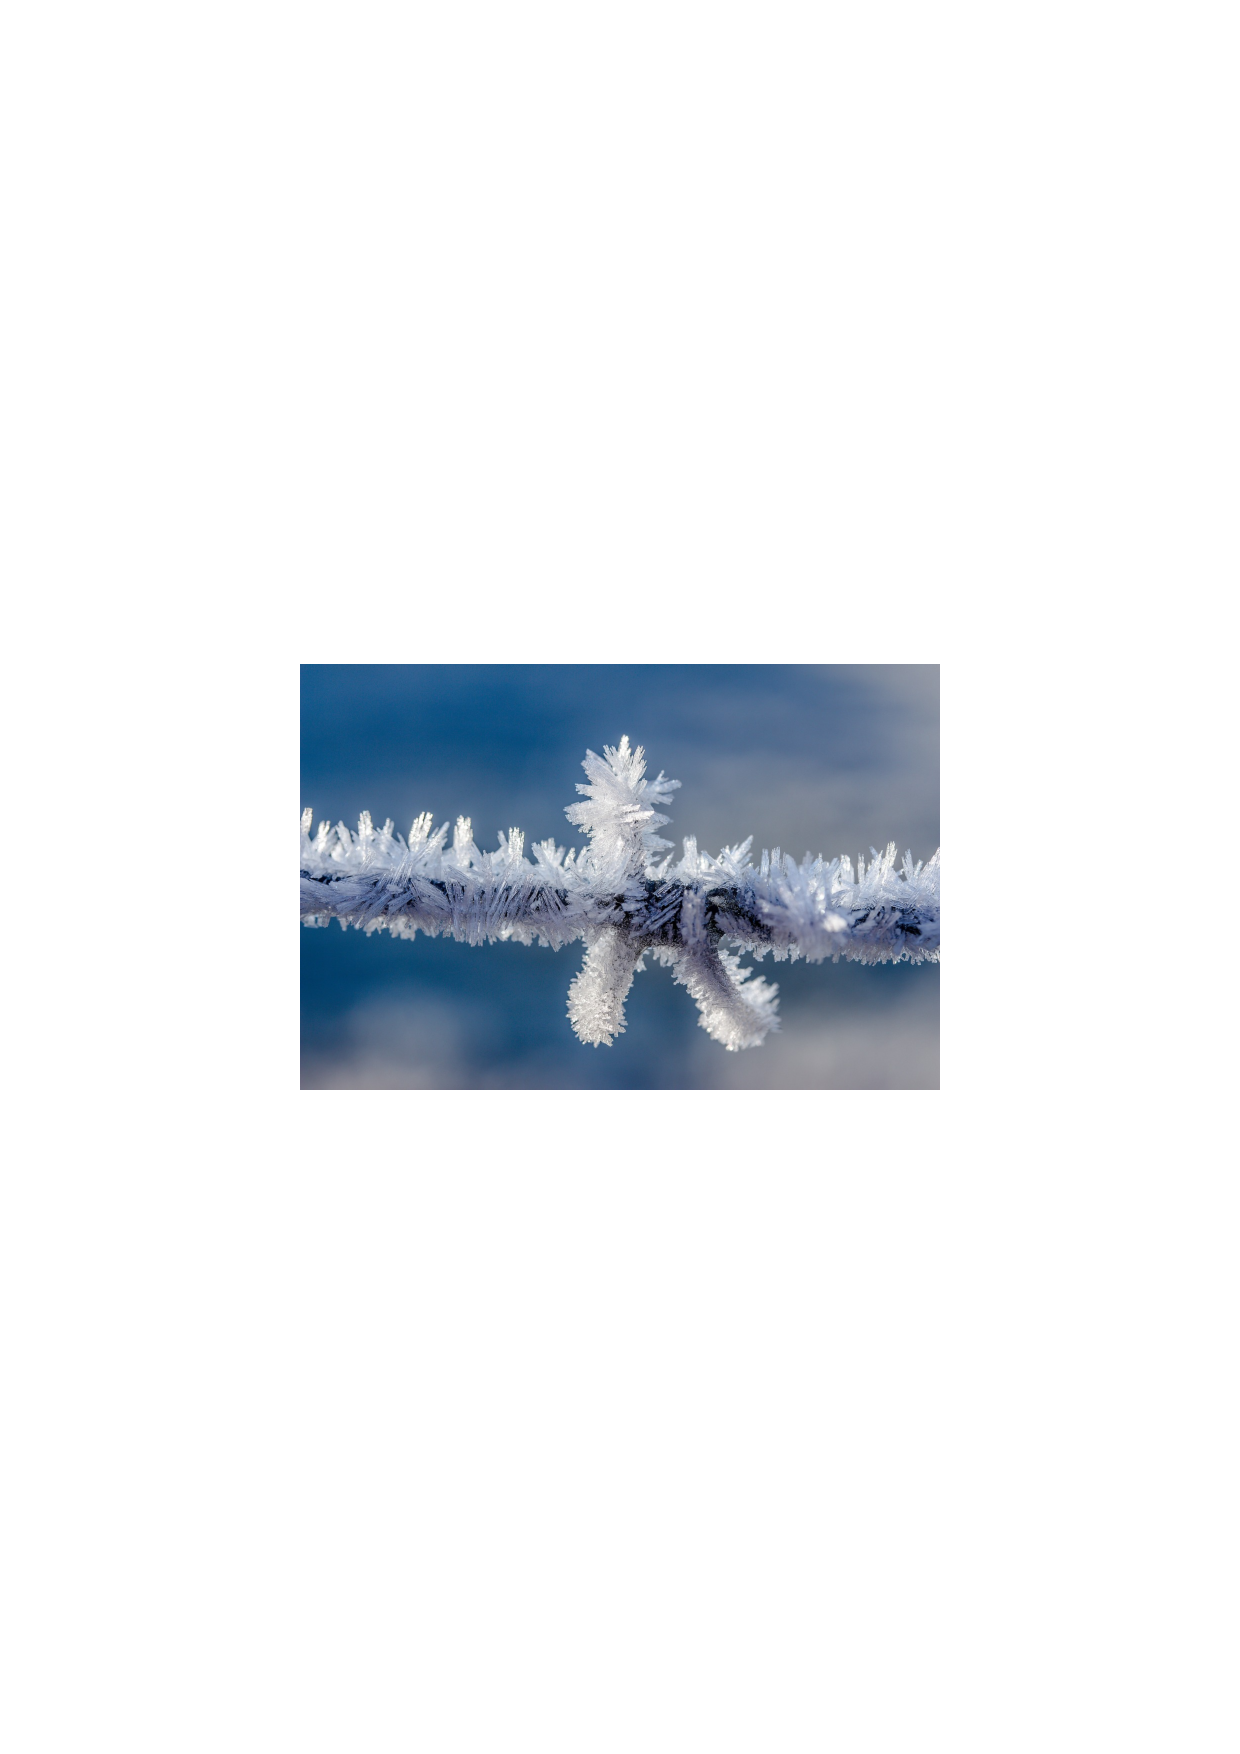
\includegraphics[width=.6\linewidth]{Chapter_1/Figs/Fig1.pdf}
	\caption[TOC Figure Description]{Caption.}
	\label{fig:Fig1}
\end{figure}
\subsubsection{This is a subsubsection}
Citations are like \cite{goossens93,AbedonHymanThomas2003}.  Or maybe \cite{Abedon1994} said something.  Or \cite{Cerveny} which is an example of how to make a bib file that includes an author whose name begins with a non-English character and \cite{forgues96}: an example of referencing a Ph.D. thesis and yet more non-English characters.




\bibliographystyle{abbrvnat}
\bibliography{Chapter_1/ref1}
